\section{Common Algorithms}

\subsection{Noise Generation}
\label{section:noise-generation}
Nature's unpredictability plays a big role in the diversity and appearance of cloudscapes. In shaders, an approach to that \textit{randomness} is used called \textit{\gls{noise}}.
In order to be able to implement random \gls{noise}, several important topics need to be looked into. It is best to start with randomness in computer science and how it is handled inside a shader program.

\subsubsection{Random Numbers}
Unfortunately, there is no magic function which returns a pure random number inside the seemingly predictable and rigid code environment.
So the question arises as to how such randomness can be generated.
\\
For this, the function $rnd(x) = fract(sin(x))$ is inspected, where $fract(x) = x - floor(x)$.

\begin{figure}[H]
    \centering
    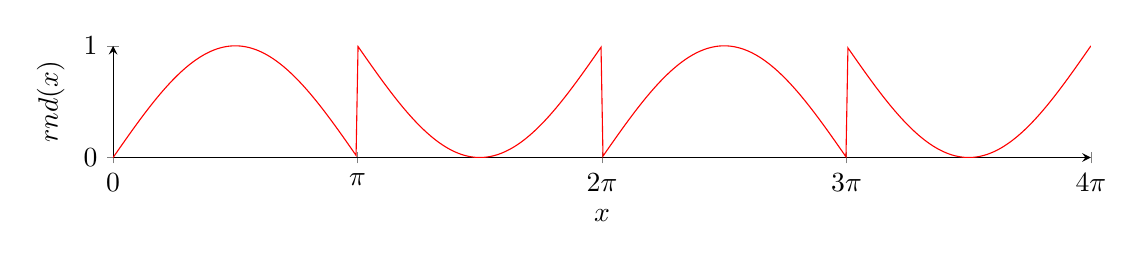
\begin{tikzpicture}[scale=1.0]
        \begin{axis}[
            samples=500,
            domain=0:4*pi,
            axis lines=left,
            xlabel=$x$,
            ylabel={$rnd(x)$},
            height=3cm,
            width=14cm,
            ytick={0,1},
            xtick={0,pi,2*pi,3*pi,4*pi},
            xticklabels={$0$,$\pi$,$2\pi$,$3\pi$,$4\pi$}
            ]
        \addplot[red] plot (\x, { sin(\x*1 r) - floor(sin(\x*1 r)) });
        \end{axis}
    \end{tikzpicture}
    \caption{Random numbers with the fractional value of sine of x.}
\end{figure}

\noindent
The sine values fluctuate between $-1.0$ and $1.0$, but with $fract$, only the fractional part is evaluated, turning the negative values into positive ones.
This effect can be used to get some pseudo-random values by "compressing" the function horizontally, or in other words by increasing the frequency of the sine wave.
\\
The next figure displays the function $rnd(x) = fract(sin(x) * 10000)$.

\begin{figure}[H]
    \centering
    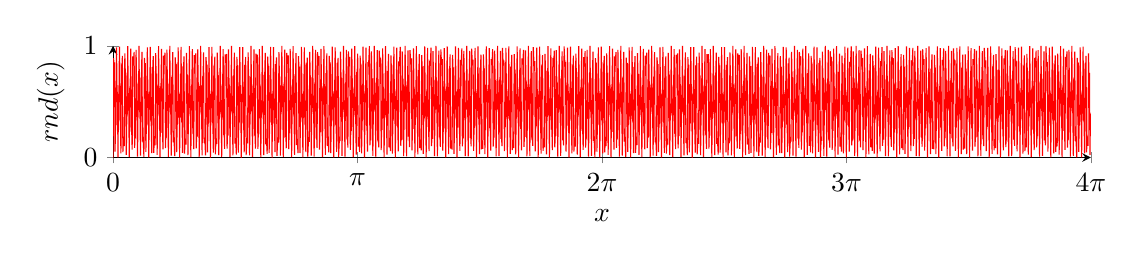
\begin{tikzpicture}[scale=1.0]
        \begin{axis}[
            samples=2000,
            domain=0:4*pi,
            axis lines=left,
            xlabel=$x$,
            ylabel={$rnd(x)$},
            height=3cm,
            width=14cm,
            ytick={0,1},
            xtick={0,pi,2*pi,3*pi,4*pi},
            xticklabels={$0$,$\pi$,$2\pi$,$3\pi$,$4\pi$},
            ]
        \addplot[red] plot (\x, { sin(\x*10000) - floor(sin(\x*10000)) });
        \end{axis}
    \end{tikzpicture}
    \caption{Random numbers with the fractional value of sine of x multiplied by 10000.}
\end{figure}

\noindent
It is clearly visible that the function $rnd(x)$ became chaotic and returns practically random values. However, it is noteworthy that $rnd(x)$ is still a deterministic function, which means for example $rnd(1.0)$ is always going to return the same value.

\clearpage
\subsubsection{2D Random}
To generate a pseudo-random number from two values instead of one, the same function can be used, with some tweaks. Those two numbers come as a two-dimensional vector, which needs to be transformed into a single floating point number.
According to Vivo, the dot product is particularily helpful in that case \cite{online:thebookofshaders}. It returns a single float value between $0.0$ and $1.0$ depending on the alignment of two vectors.
They describe the following method:

\begin{lstlisting}[language=HLSL, caption=Implementation of 2D random number generation., label=lst:random:2d]
float random2d(float2 co) {
    return fract(sin(dot(co, float2(12.9898,78.233))) * 43758.5453123);
}
\end{lstlisting}

\noindent
When using the fragment coordinates as the vector \lstinline[language=HLSL]{co} and calls \lstinline[language=HLSL]{random2d(co)} for every pixels, the resulting image shows a seemingly random assortment of pixels holding values from 0 to 1 (from black to white).

\begin{figure}[H]
    \centering
            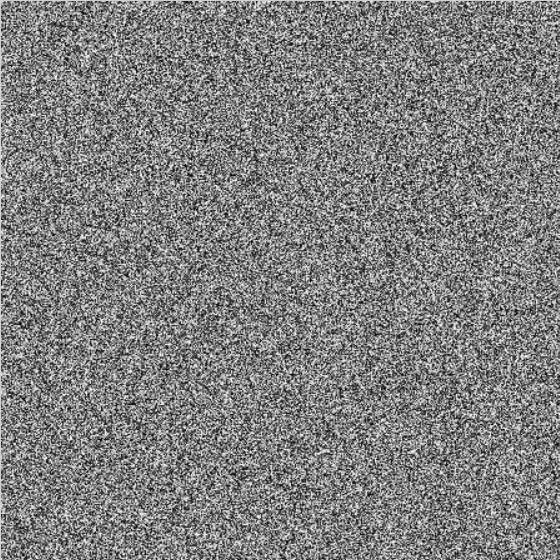
\includegraphics[width=0.45\linewidth]{noise/2d random}
            \captionof{figure}{2D random function visualized.}
            \label{img:noise:2d:random}
\end{figure}

This method of procedural randomness still has one major flaw: It has no patterns. Contratictory to the word "random", a certain pattern is required in order to generate \textit{random} clouds. Luckily, there is more to random generation than just a highly sped up sine wave.
